\documentclass[aspectratio=169, 10pt]{beamer}

% Professional Theme Setup
\usetheme{Boadilla}
\usecolortheme{dove}
\usefonttheme{professionalfonts}

% Packages
\usepackage{graphicx}
\usepackage{hyperref}
\usepackage{booktabs}
\usepackage{xcolor}
\usepackage{tikz}
\usepackage{tabularx}
\usepackage{fontawesome5} % For professional icons

% Corporate Brand Colors
\definecolor{CorporatePrimary}{HTML}{1E293B} % Slate 800
\definecolor{CorporateSecondary}{HTML}{4F46E5} % Indigo 600
\definecolor{CorporateAccent}{HTML}{0EA5E9} % Sky 500
\definecolor{LightGray}{HTML}{F8FAFC} % Slate 50

% Beamer Color Assignments
\setbeamercolor{palette primary}{bg=CorporatePrimary,fg=white}
\setbeamercolor{palette secondary}{bg=CorporateSecondary,fg=white}
\setbeamercolor{palette tertiary}{bg=CorporateAccent,fg=white}
\setbeamercolor{title}{fg=CorporatePrimary}
\setbeamercolor{frametitle}{bg=CorporatePrimary,fg=white}
\setbeamercolor{itemize item}{fg=CorporateSecondary}
\setbeamercolor{itemize subitem}{fg=CorporateAccent}
\setbeamercolor{section in toc}{fg=CorporatePrimary}

% Formatting
\setbeamertemplate{navigation symbols}{}
\setbeamertemplate{itemize items}[circle]
\setbeamertemplate{footline}[frame number]

\title{\LARGE AwardX}
\subtitle{\vspace{0.2cm}\large The Next-Generation Enterprise Platform for Awards, Grants, and Competitions}
\author{\vspace{0.5cm}\textbf{Confidential Investor Presentation}}
\date{\small April 2026}

\begin{document}

{
\setbeamertemplate{footline}{}
\begin{frame}
    \titlepage
\end{frame}
}

\begin{frame}{Executive Summary}
    \begin{columns}[T]
        \column{0.48\textwidth}
        \textbf{\textcolor{CorporateSecondary}{\faBullseye \quad The Opportunity}}
        \vspace{0.2cm}\\
        The \$2.5B+ grants and awards management industry relies on legacy, fragmented software. High friction in application processes results in up to 40\% applicant drop-off, while administrators lose hundreds of hours to manual data entry and disjointed judging workflows.
        
        \vspace{0.5cm}
        \textbf{\textcolor{CorporateSecondary}{\faRocket \quad The Solution}}
        \vspace{0.2cm}\\
        AwardX is a multi-tenant, cloud-native SaaS platform designed to unify the entire lifecycle of awards and competitions. We combine consumer-grade UX, AI-assisted scoring, and enterprise-grade infrastructure to reduce operational overhead by 70\%.
        
        \column{0.48\textwidth}
        \textbf{\textcolor{CorporateSecondary}{\faChartLine \quad Key Metrics \& Ask}}
        \vspace{0.2cm}
        \begin{itemize}
            \item \textbf{Target Market:} \$800M SAM in North America and Europe.
            \item \textbf{Revenue Model:} Tiered B2B SaaS + Payment Processing Take-Rate.
            \item \textbf{Technical Moat:} Sub-1.5s LCP, built on React 19, Supabase, and Vercel Edge.
            \item \textbf{Funding Ask:} \$1.5M Seed round to scale Go-To-Market execution and launch proprietary AI-scoring modules.
        \end{itemize}
    \end{columns}
\end{frame}

\begin{frame}{The Problem: A Broken \& Fragmented Ecosystem}
    Organizations running awards and grants currently force their users through a disjointed, frustrating ecosystem.
    
    \vspace{0.4cm}
    \begin{columns}[T]
        \column{0.3\textwidth}
        \textbf{For Administrators}
        \begin{itemize}
            \item \small Over-reliance on "duct-taped" solutions (Typeform + Sheets + Email).
            \item \small No centralized audit trails or secure RBAC (Role-Based Access Control).
            \item \small High administrative burden for onboarding judges.
        \end{itemize}
        
        \column{0.3\textwidth}
        \textbf{For Applicants}
        \begin{itemize}
            \item \small Clunky, inaccessible forms lacking dynamic validation.
            \item \small Inability to save drafts effectively across sessions.
            \item \small High abandonment rates leading to reduced program revenue.
        \end{itemize}
        
        \column{0.3\textwidth}
        \textbf{For Judges}
        \begin{itemize}
            \item \small Reviewing sensitive documents via unsecure email attachments.
            \item \small Disconnected scoring rubrics.
            \item \small Lack of contextual comparison and collaboration tools.
        \end{itemize}
    \end{columns}
\end{frame}

\begin{frame}{The Solution: The AwardX Ecosystem}
    AwardX centralizes the entire lifecycle into a single, cohesive, and highly performant platform.
    \vspace{0.4cm}
    
    \begin{itemize}
        \item \textbf{\textcolor{CorporateSecondary}{Intelligent Program Builder:}} Launch complex, multi-stage programs in under 15 minutes utilizing a drag-and-drop builder with conditional logic and automated workflows.
        \vspace{0.2cm}
        \item \textbf{\textcolor{CorporateSecondary}{Frictionless Applicant Portal:}} A responsive, beautifully designed interface featuring real-time auto-saving, inline validation, and embedded payment gateways (Stripe Connect \& Razorpay).
        \vspace{0.2cm}
        \item \textbf{\textcolor{CorporateSecondary}{Secure, Tokenized Judging:}} Passwordless, secure portal access for external reviewers. Features side-by-side asset viewing and dynamic scoring rubrics, eventually powered by Gemini AI for contextual scoring assistance.
        \vspace{0.2cm}
        \item \textbf{\textcolor{CorporateSecondary}{Real-time Analytics \& CRM:}} Comprehensive dashboard offering actionable insights into submission velocity, geographic distribution, and revenue generation.
    \end{itemize}
\end{frame}

\begin{frame}{Technological Moat \& Architecture}
    We are not just building another form builder; we are engineering an enterprise-grade operating system.
    
    \vspace{0.4cm}
    \begin{table}[]
        \centering
        \renewcommand{\arraystretch}{1.5}
        \begin{tabularx}{\textwidth}{l X}
            \toprule
            \textbf{Pillar} & \textbf{Implementation \& Advantage} \\
            \midrule
            \textbf{Performance} & Edge-hosted via Vercel with React 19. Achieving sub-1.5s Largest Contentful Paint (LCP), maximizing applicant conversion. \\
            \textbf{Security} & Deep integration with Supabase. Strict Row-Level Security (RLS) ensures multi-tenant data isolation and compliance. \\
            \textbf{Extensibility} & API-first design architecture. Seamlessly handles complex data relationships (categories, rounds, judging criteria) via robust PostgreSQL schema. \\
            \textbf{Intelligence} & Integration roadmap for Google Gemini API to provide automated submission summaries and bias-detection in scoring. \\
            \bottomrule
        \end{tabularx}
    \end{table}
\end{frame}

\begin{frame}{Market Opportunity}
    The digital transformation of administrative workflows in non-profits, academia, and enterprise is accelerating.
    
    \vspace{0.3cm}
    \begin{columns}
        \column{0.4\textwidth}
        \begin{center}
            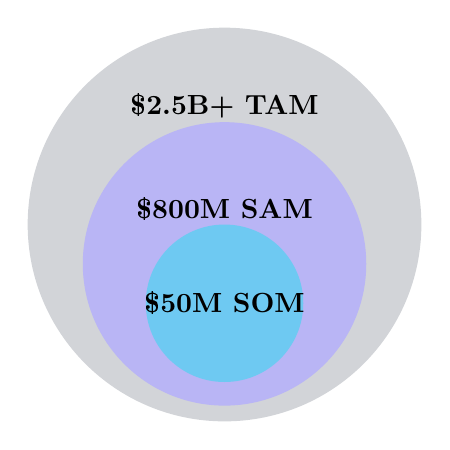
\begin{tikzpicture}
                \fill[CorporatePrimary!20] (0,0) circle (2.5);
                \fill[CorporateSecondary!40] (0,-0.5) circle (1.8);
                \fill[CorporateAccent!60] (0,-1) circle (1.0);
                
                \node at (0, 1.5) {\textbf{\$2.5B+ TAM}};
                \node at (0, 0.2) {\textbf{\$800M SAM}};
                \node at (0, -1) {\textbf{\$50M SOM}};
            \end{tikzpicture}
        \end{center}
        
        \column{0.55\textwidth}
        \textbf{Target Segments:}
        \begin{itemize}
            \item \textbf{Industry Associations:} Managing annual excellence awards.
            \item \textbf{Academia \& Research:} Processing grant applications and scholarships.
            \item \textbf{Enterprise HR:} Internal employee recognition and innovation challenges.
        \end{itemize}
        \vspace{0.3cm}
        \textbf{Market Tailwinds:}
        \begin{itemize}
            \item Increased demand for data security and compliance (GDPR/CCPA).
            \item Expectation of consumer-grade UX in B2B software.
        \end{itemize}
    \end{columns}
\end{frame}

\begin{frame}{Business \& Revenue Model}
    A highly scalable, dual-engine revenue model designed for high Net Revenue Retention (NRR).
    
    \vspace{0.4cm}
    \begin{columns}[T]
        \column{0.48\textwidth}
        \textbf{1. B2B SaaS Subscriptions}
        \vspace{0.2cm}
        \begin{itemize}
            \item \textbf{Starter (\$99/mo):} Single program, core features, standard support.
            \item \textbf{Pro (\$299/mo):} Unlimited programs, advanced analytics, custom domain routing, priority support.
            \item \textbf{Enterprise (Custom):} White-labeling, dedicated account management, custom SLA, and SSO integrations.
        \end{itemize}
        
        \column{0.48\textwidth}
        \textbf{2. Transactional Revenue}
        \vspace{0.2cm}
        \begin{itemize}
            \item Many awards and competitions charge application or entry fees.
            \item AwardX processes these via Stripe Connect and Razorpay.
            \item We capture a \textbf{1.5\% - 3.0\% take-rate} on all processed entry fees, creating uncapped revenue upside tied directly to our clients' success.
        \end{itemize}
    \end{columns}
\end{frame}

\begin{frame}{Competitive Landscape}
    \begin{table}[]
        \centering
        \renewcommand{\arraystretch}{1.4}
        \begin{tabularx}{\textwidth}{l c c c c}
            \toprule
            \textbf{Capability} & \textbf{AwardX} & \textbf{Zelous} & \textbf{Awardforce} & \textbf{Generic Forms} \\
            \midrule
            Modern, Consumer-Grade UX & \textcolor{CorporateSecondary}{\faCheckCircle} & \textcolor{gray}{\faCircle} & \textcolor{gray}{\faTimesCircle} & \textcolor{CorporateSecondary}{\faCheckCircle} \\
            End-to-End Workflow & \textcolor{CorporateSecondary}{\faCheckCircle} & \textcolor{CorporateSecondary}{\faCheckCircle} & \textcolor{CorporateSecondary}{\faCheckCircle} & \textcolor{gray}{\faTimesCircle} \\
            AI-Assisted Processing & \textcolor{CorporateSecondary}{\faCheckCircle} (Planned) & \textcolor{gray}{\faTimesCircle} & \textcolor{gray}{\faTimesCircle} & \textcolor{gray}{\faTimesCircle} \\
            Sub-Second Performance & \textcolor{CorporateSecondary}{\faCheckCircle} & \textcolor{gray}{\faTimesCircle} & \textcolor{gray}{\faTimesCircle} & \textcolor{CorporateSecondary}{\faCheckCircle} \\
            Tokenized, Passwordless Judging & \textcolor{CorporateSecondary}{\faCheckCircle} & \textcolor{gray}{\faCircle} (Clunky) & \textcolor{CorporateSecondary}{\faCheckCircle} & \textcolor{gray}{\faTimesCircle} \\
            White-Label Customization & \textcolor{CorporateSecondary}{\faCheckCircle} & \textcolor{CorporateSecondary}{\faCheckCircle} & \textcolor{gray}{\faCircle} & \textcolor{gray}{\faTimesCircle} \\
            \bottomrule
        \end{tabularx}
    \end{table}
    \vspace{0.2cm}
    \textit{\small *Generic Forms includes Typeform, Google Forms, SurveyMonkey.}
\end{frame}

\begin{frame}{Go-to-Market (GTM) Strategy}
    Our initial growth relies on targeted outbound sales and a robust Product-Led Growth (PLG) viral loop.
    
    \vspace{0.4cm}
    \begin{itemize}
        \item \textbf{Direct Outbound (Months 1-6):} Targeting mid-market trade associations and event organizers. Utilizing personalized outreach demonstrating ROI through reduced administrative hours.
        \vspace{0.2cm}
        \item \textbf{Partnerships \& Channels (Months 6-12):} Partnering with event management agencies and PR firms who run awards on behalf of their corporate clients.
        \vspace{0.2cm}
        \item \textbf{The PLG Viral Loop:} Every applicant and judge exposed to the AwardX platform experiences its superior UX. "Powered by AwardX" branding on Starter tier forms drives inbound leads from participants who run their own programs.
    \end{itemize}
\end{frame}

\begin{frame}{Development Roadmap \& Milestones}
    \begin{columns}[T]
        \column{0.48\textwidth}
        \textbf{H1 2026: Foundation \& Core}
        \begin{itemize}
            \item \textbf{Phase 1:} Architecture hardening, comprehensive RLS security implementation, and performance optimization (achieving <1.5s LCP).
            \item \textbf{Phase 2:} Release of the core engine: drag-and-drop form builder, multi-stage rounds, real-time sync, and tokenized judge portal.
        \end{itemize}
        
        \column{0.48\textwidth}
        \textbf{H2 2026: Growth \& Scale}
        \begin{itemize}
            \item \textbf{Phase 3:} Integration of Stripe Connect for payment processing, custom domains (white-labeling), and the launch of the Gemini AI Scoring Assistant.
            \item \textbf{Phase 4:} Enterprise scalability (Redis caching, materialized views for advanced analytics), Playwright E2E testing, and SOC2 compliance preparation.
        \end{itemize}
    \end{columns}
\end{frame}

\begin{frame}{Financial Projections (3-Year Outlook)}
    \begin{center}
        \renewcommand{\arraystretch}{1.5}
        \begin{tabular}{lccc}
            \toprule
            \textbf{Metric} & \textbf{Year 1} & \textbf{Year 2} & \textbf{Year 3} \\
            \midrule
            Active Organizations & 150 & 600 & 2,000+ \\
            SaaS ARR & \$350K & \$1.8M & \$6.5M \\
            Gross Transaction Volume (GTV) & \$2.0M & \$15.0M & \$60.0M \\
            Transactional Revenue (2\% avg) & \$40K & \$300K & \$1.2M \\
            \textbf{Total Gross Revenue} & \textbf{\$390K} & \textbf{\$2.1M} & \textbf{\$7.7M} \\
            \bottomrule
        \end{tabular}
    \end{center}
    \vspace{0.3cm}
    \textit{\small Assumptions: ACV of \~\$2,400. Transaction volume scales as organizations run larger, premium programs.}
\end{frame}

\begin{frame}{The Ask \& Use of Funds}
    \textbf{\Large Raising \$1.5M Seed Round}
    
    \vspace{0.4cm}
    \begin{columns}
        \column{0.5\textwidth}
        \textbf{Fund Allocation}
        \begin{itemize}
            \item \textbf{50\% Product \& Engineering:} Accelerate the development of the AI Scoring Assistant, robust automation rules, and mobile-native experiences.
            \item \textbf{35\% Sales \& Marketing:} Build out the direct sales team, fund targeted ABM (Account-Based Marketing) campaigns, and establish presence at key industry conferences.
            \item \textbf{15\% Operations \& Legal:} Infrastructure scaling, security audits, and legal framework for global payment processing.
        \end{itemize}
        
        \column{0.45\textwidth}
        \textbf{Key Milestones (18 Months)}
        \begin{itemize}
            \item Reach \$1M+ in ARR.
            \item Process >\$5M in entry fee volume.
            \item Secure 3-5 flagship enterprise clients to establish market authority.
            \item Prepare for Series A scale-up.
        \end{itemize}
    \end{columns}
\end{frame}

\begin{frame}{Contact \& Next Steps}
    \begin{center}
        \Huge \textbf{AwardX} \\
        \vspace{0.8cm}
        \Large \textcolor{CorporateSecondary}{Transforming how the world manages and recognizes excellence.} \\
        \vspace{1cm}
        \normalsize 
        \textbf{Contact us to request access to the data room:} \\
        \vspace{0.2cm}
        investors@awardx.com \\
        www.awardx.com \\
        \vspace{0.5cm}
        \textit{Thank you for your time.}
    \end{center}
\end{frame}

\end{document}
